% !TeX program = xelatex
\documentclass[conference]{IEEEtran}
\IEEEoverridecommandlockouts

\usepackage{cite}
\usepackage{amsmath,amssymb,amsfonts}
\usepackage{array}
\usepackage{booktabs}
\usepackage{graphicx}
\usepackage[hidelinks]{hyperref}
\usepackage{placeins}
\usepackage{textcomp}
\usepackage{xcolor}
\usepackage{xeCJK}
\setCJKmainfont{Noto Serif CJK SC}
\setCJKsansfont{Noto Sans CJK SC}
\setCJKmonofont{Noto Sans Mono CJK SC}
\setmainfont{DejaVu Serif}
\setsansfont{DejaVu Sans}
\setmonofont{DejaVu Sans Mono}
\XeTeXlinebreaklocale "zh"
\XeTeXlinebreakskip = 0pt plus 1pt
\renewcommand{\abstractname}{摘\quad 要}
\renewcommand{\IEEEkeywordsname}{关键词}

\setlength{\textfloatsep}{4pt plus 1pt minus 1pt}
\setlength{\floatsep}{3pt plus 1pt minus 1pt}
\setlength{\intextsep}{4pt plus 1pt minus 1pt}
\setlength{\abovecaptionskip}{2pt}
\setlength{\belowcaptionskip}{1pt}

\begin{document}

\title{面向覆盖率的规划器引导记忆残差强化学习方法：机器人热斑覆盖研究}

\author{\IEEEauthorblockN{蒋健，毛轶海*}
\IEEEauthorblockA{\textit{中国科学院沈阳计算技术研究所}，沈阳，中国\\
\textit{中国科学院大学}，北京，中国\\
449192322@qq.com, myhfree@126.com}
\thanks{*通信作者：毛轶海。}}

\maketitle

\begin{abstract}
固态白酒蒸馏上甑过程中，局部蒸汽突破位置提示酒醅的后续投放区域。本文在ABB机械臂的MuJoCo数字孪生环境中研究相应的持续服务控制问题：外部热定位模块提供聚集分布的目标位置，机械臂驱动抽象铺料中心服务活动热斑。Horizon-2滚动时域规划器提供结构化动作先验，LSTM-PPO策略依据活动目标集合、生成历史、热场上下文和路线摘要学习带阶段缩放及进度保护的有界残差。实验采用3个训练种子、3个留出环境种子，并在每个交叉单元运行5个回合。相较Horizon-2，本方法在Low、Realistic和Hard阶段的覆盖率无统计可区分差异；Extreme阶段由0.816提高至0.855，差值的分层95\%置信区间为$[0.003,0.074]$，但经四阶段Holm校正后不显著。保留编码器、H2行为克隆预热、预测损失和服务奖励的匹配绝对动作消融，使四阶段覆盖率降低0.079--0.168。Extreme阶段的覆盖率增加同时伴随更高延迟与积压。因此，本方法体现的是以覆盖率为主的规划--学习权衡，而非统一更快的控制器。
\end{abstract}

\begin{IEEEkeywords}
机器人覆盖，残差强化学习，持续服务，覆盖路径规划，LSTM-PPO，MuJoCo
\end{IEEEkeywords}

\begin{figure*}[t]
\centering
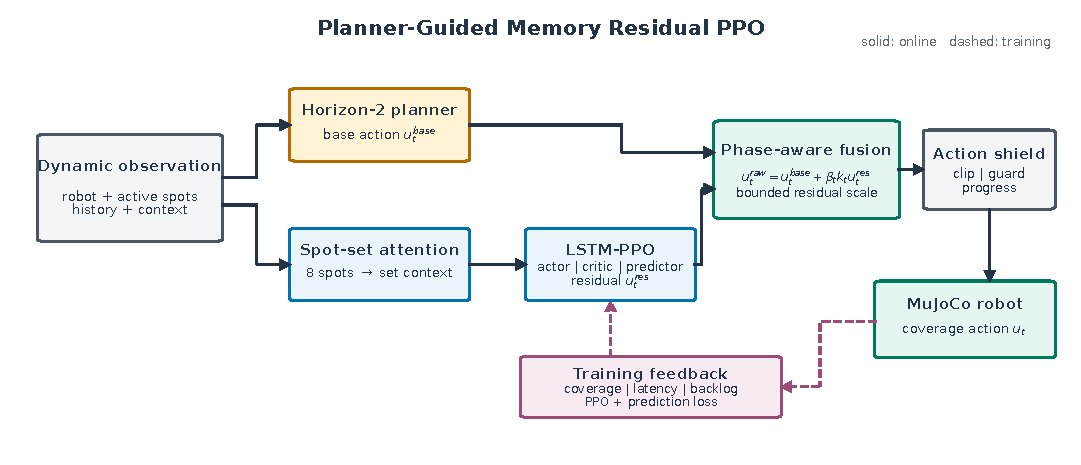
\includegraphics[width=0.86\textwidth]{figures/method_framework.pdf}
\caption{规划器引导的残差控制框架。在线规划器始终位于动作回路内；LSTM-PPO给出有界修正，进度保护器在动作发送至MuJoCo机械臂前检查局部进展。}
\label{fig:framework_zh}
\end{figure*}

\section{引言}
上甑是固态白酒蒸馏的重要工序~\cite{wang2024baijiu}，作业人员依据蒸汽突破位置实施“见气即洒”，并维持酒醅轻薄、均匀的铺层。响应不及时或投放不一致可能导致压汽、串汽、漏料及铺层不均。本文研究其自动化控制抽象：外部热感知系统给出蒸汽突破坐标，ABB机械臂移动铺料中心服务活动位置。目标以空间聚集的爆发--沉寂周期到达，在被覆盖前持续存在，并可能在机械臂运动过程中积累，因而需要联合考虑几何行程、等待时间、目标年龄和队列拥塞。

本文只验证已知目标坐标条件下的在线路径决策与运动指令，不评价红外图像检测精度、酒醅材料动力学、铺层均匀性和最终蒸馏质量。因此，仿真中的一次覆盖表示对已检测蒸汽突破位置的服务，不等同于完整上甑工艺已经得到实证验证。

该问题与覆盖路径规划~\cite{galceran2013survey}、覆盖控制~\cite{cortes2004coverage}、统计覆盖~\cite{arslan2019statistical}、随机到达下的持续监测~\cite{yu2015persistent}以及随机动态车辆路径问题~\cite{bertsimas1991stochastic,bertsimas1993multiple}相关。与静态区域覆盖不同，活动热斑仅在物理覆盖后离开队列。已有研究将强化学习用于自适应覆盖~\cite{carvalho2025zeroshot,champagnie2024online}；然而，在目标位置可见时，确定性规划器本身已构成有竞争力的先验。残差强化学习~\cite{johannink2019residual}及有界残差控制~\cite{yan2025ictrl,zhang2023robodact}能够在保留该先验的同时学习局部修正，集合编码器则遵循Set Transformer的置换不变思想~\cite{lee2019settransformer}。

本文主要对应ICCC Track 6（Robotics），并与Track 2（AI for Engineering）和Track 4（Machine Learning）相关。研究问题为：\emph{RQ1}，相较匹配的绝对动作PPO控制器，有界规划残差接口能否提高固定规划器的性能；\emph{RQ2}，该方法与其他规划器及启发式先验相比如何；\emph{RQ3}，其在延迟、严格SLA、积压和平滑度上形成何种覆盖率--服务代价权衡。

本文不以学习替代规划，而是在在线路线先验周围学习修正。主要贡献包括：（1）给出指标分母明确的持续热斑服务建模；（2）构建具有阶段化残差权限和进度保护的LSTM-PPO接口；（3）采用交叉留出评估，将残差动作接口的证据与辅助模块作用区分开来。

\section{任务与方法}
\subsection{持续服务与评价指标}
设活动热斑集合为$\mathcal S_t=\{p_i(t)\}$，其中$p_i=(x_i,y_i,a_i)$表示位置与活动年龄，覆盖中心为$c_t=(x_t,y_t)$。当
\begin{equation}
\|c_t-(x_i,y_i)\|_2\le r_{\mathrm{cover}}
\end{equation}
时，热斑$i$完成服务并被移除。报告实验禁用超时移除，因此未覆盖热斑仍计入分母。动作$u_t=[\Delta x_t,\Delta y_t,s_t]\in[-1,1]^3$每$0.05$ s下发一次，MuJoCo物理积分步长为$0.002$ s。覆盖率定义为
\begin{equation}
C=N_{\mathrm{covered}}/N_{\mathrm{spawned}}.
\end{equation}
对已覆盖热斑，响应时间为$T_i=(n_i^{\mathrm{cover}}-n_i^{\mathrm{spawn}})\times0.05$ s，平均延迟为$\bar T=N_{\mathrm{covered}}^{-1}\sum_iT_i$。平均值和p90均以已覆盖热斑为条件，p90为单回合延迟列表的经验90百分位数。严格SLA定义为
\begin{equation}
C_{\mathrm{SLA}}=\frac{|\{i:T_i\le T_{\mathrm{SLA}}\}|}{N_{\mathrm{spawned}}},
\qquad T_{\mathrm{SLA}}=4.0\ \mathrm{s}.
\end{equation}
积压为时间平均活动热斑数；平滑度为$\Delta_u=T^{-1}\sum_t\|u_t-u_{t-1}\|_2$。统计重采样前先在评估单元内聚合，覆盖率为主要指标。

\subsection{规划先验与循环残差}
风险感知比较器使用
\begin{equation}
q_i=0.40\phi_{\mathrm{age}}+0.30\phi_{\mathrm{dist}}
 +0.10\phi_{\mathrm{reach}}+0.20\phi_{\mathrm{therm}}.
\end{equation}
各分量为
\begin{align}
\phi_{\mathrm{age}}&=\operatorname{clip}(a_i/A_{\mathrm{norm}},0,1),\nonumber\\
\phi_{\mathrm{dist}}&=1-\operatorname{clip}(\|p_i-c_t\|/R_{\mathrm{pot}},0,1),\nonumber\\
\phi_{\mathrm{reach}}&=1-\operatorname{clip}(\|p_i-p_{\mathrm{home}}\|/R_{\max},0,1),\nonumber\\
\phi_{\mathrm{therm}}&=\operatorname{clip}(H(p_i),0,1).
\end{align}
材料缺口分量为$\phi_{\mathrm{mat}}=\operatorname{clip}(\operatorname{mean}_g[\max(H^*-H_g,0)\exp(-\|x_g-p_i\|^2/(2\sigma_d^2))]/H^*,0,1)$，其中$\sigma_d=0.18$ m。热场分数为$H(p)=\operatorname{clip}(\sum_\ell a_\ell\exp(-\|p-h_\ell\|^2/(2\sigma_h^2)),0,1)$，$\sigma_h=0.22$ m。启用材料观测时，年龄、距离、材料、可达性和热场权重为$(.35,.25,.15,.10,.15)$；评估协议不使用材料观测及可选紧迫度增强，故实际权重为$(.40,.30,0,.10,.20)$。风险感知启发式无隐状态，选择活动集合中首个取得最大$q_i$的热斑，并以速度1输出指向该目标的归一化方向。

Horizon-$L$枚举长度为$\min(L,N_t)$的有序路线。对$\rho=(i_1,\ldots,i_L)$，规划器模拟行程并计算
\begin{align}
g_j &= q_{i_j}+0.45z_j-0.018d_j-0.050(z_j-1)_+,\nonumber\\
J(\rho) &= \sum_{j=1}^{L}0.82^{j-1}g_j-0.08\bar z_{\mathrm{left}},
\end{align}
其中$d_j$为行程步数，$z_j$为以$A_{\mathrm{norm}}$归一化的预计到达年龄；每个路线元素后更新模拟中心和累计行程。H2取$L=2$，H3取$L=3$。规划器枚举全部有序路线，使用$d_j=\max(1,\lceil\max(\|p_{i_j}-c\|-r_{\mathrm{cover}},0)/0.04\rceil)$，完全并列时保留首个枚举路线，并仅执行最高分路线的首个动作。环境随后应用$\bar u_t=0.7\bar u_{t-1}+0.3\tilde u_t$；平面位移为$0.04\eta_t[d_x,d_y]$，其中$\eta_t=0.65+0.35(d_s+1)/2$。

\begin{table}[t]
\caption{Horizon-2目标选择流程}
\label{tab:h2algorithm_zh}
\centering\scriptsize
\begin{tabular}{@{}p{0.96\columnwidth}@{}}
\toprule
\textbf{输入：}活动集合$\mathcal S_t$、覆盖中心$c_t$和$L=2$。\\
1. 枚举$\mathcal R_t=\operatorname{Perm}(\mathcal S_t,\min(2,|\mathcal S_t|))$并计算各路线$J(\rho)$。\\
2. 令$\rho^*=\arg\max J(\rho)$；严格大于比较使并列时保持枚举顺序。\\
3. 输出指向$p_{\rho^*_1}$的归一化方向及速度1，并裁剪至$[-1,1]^3$。\\
4. 下一决策步重新规划，不传递规划器隐状态。\\
\bottomrule
\end{tabular}
\end{table}

观测由$61+8\times8=125$维特征组成。全局分支为$61\rightarrow256$；8个热斑槽经共享的$8\rightarrow128$映射和4头掩码注意力编码，再由$128\rightarrow256$映射；拼接特征通过$512\rightarrow256\rightarrow256$融合层进入单层、宽度256的LSTM。共享循环表征连接$256\rightarrow3$策略头、$256\rightarrow1$价值头及$256\rightarrow128\rightarrow2$预测头。策略均值使用tanh，状态无关的对数标准差初始化为$-0.8$。相对坐标和距离按甑锅半径缩放，年龄按$A_{\mathrm{norm}}$缩放；关节量和末端跟踪误差保留仿真单位，不使用测试集运行归一化器。隐状态跨采样分块和覆盖事件传递，在遗漏事件和回合边界重置。

给定规划动作$u_t^{\mathrm{base}}$和残差$u_t^{\mathrm{res}}=\pi_\theta(o_t,h_t)$，候选动作为
\begin{align}
\tilde u_t&=\operatorname{clip}(u_t^{\mathrm{base}}+\beta_tk_tu_t^{\mathrm{res}},-1,1),\nonumber\\
\beta_t&=0.03+0.17\operatorname{clip}(n_t/700000,0,1).
\end{align}
沉寂、稀疏、积累、中等、密集和爆发阶段的$k_t$分别为$(1.35,1.25,1.00,1.00,0.40,0.25)$。保护器拒绝方向一致性低于$0.15$的动作，要求候选进展至少达到基准进展的$0.35$且容差为$0.002$；保护混合为$0.70$基准加$0.30$候选，并保留至少$0.50$基准进展。转向余弦低于$-0.55$时进行混合，连续90步未覆盖后拒绝比基准更差的候选。该机制是局部进度过滤器，不构成形式化时序逻辑安全保证~\cite{alshiekh2018shielding}。

标量奖励包含时间、活动数、平均年龄、势函数、最佳进展、覆盖、快速覆盖、精度、延迟、最老目标、积压、SLA、动作变化、动作范数、遗漏和成功项。四阶段覆盖、快速覆盖和势函数基础值分别为$(68,64,62,60)$、$(16,14,12,10)$和$(8.0,7.5,6.5,5.8)$；对应缩放系数为$(.70,3.0,.65,.65,.45,2.4,2.8)$。其余系数为$r_{\mathrm{time}}=(.030,.035,.045,.055)$、$r_{\mathrm{latency}}=30$、$r_{\mathrm{oldest}}=.45$、$r_{\mathrm{backlog}}=.20$、$r_{\mathrm{SLA}}=(20,-30)$、$r_{\Delta u}=.025$、$r_{\|u\|}=.004$、$r_{\mathrm{miss}}=28$和$r_{\mathrm{success}}=30$。由于关闭超时移除，遗漏项不激活。总奖励乘$0.02$并裁剪至$[-4,4]$；SLA和积压因此属于标量偏好而非硬约束。

\begin{figure}[t]
\centering
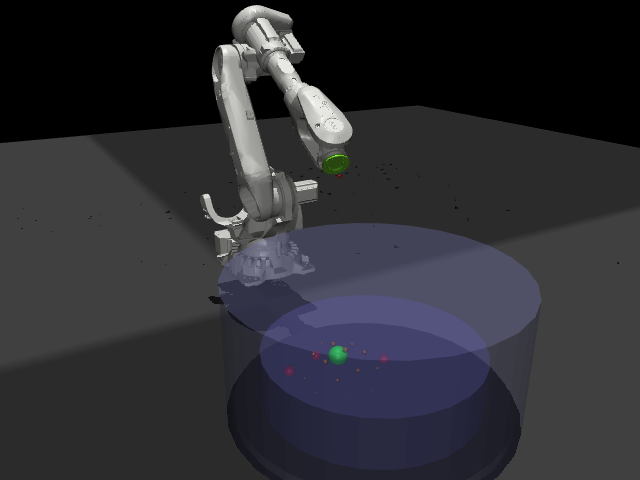
\includegraphics[width=0.37\columnwidth]{figures/mujoco_environment_snapshot.png}\hfill
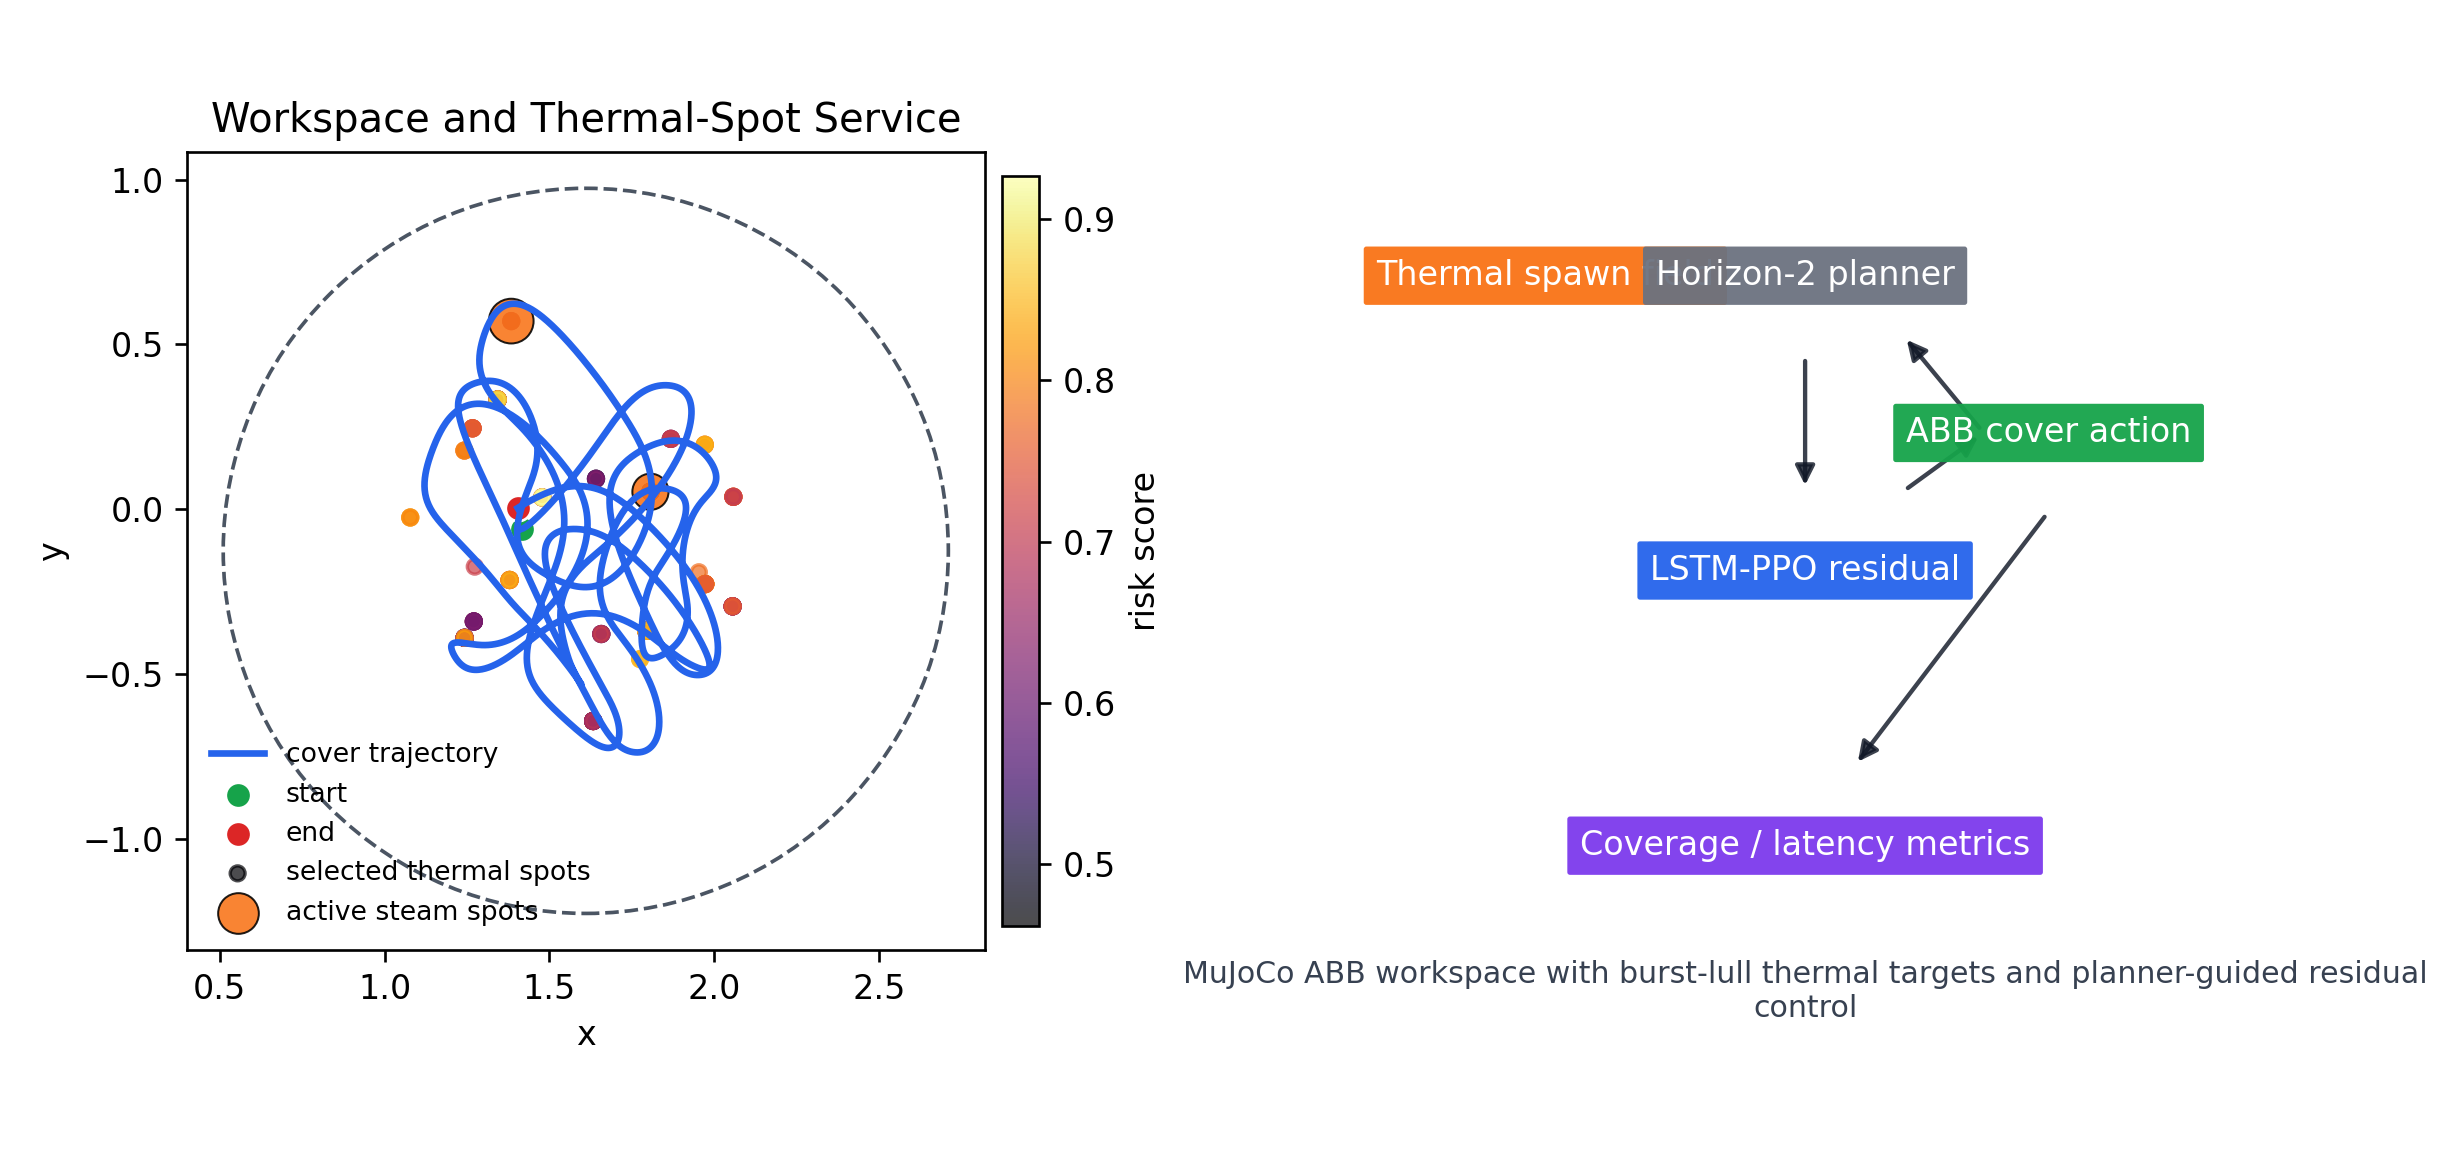
\includegraphics[width=0.60\columnwidth]{figures/mujoco_task_overview.png}
\caption{MuJoCo ABB工作空间（左）与在线热斑服务任务（右）。控制器在圆形甑锅内移动绿色覆盖中心。}
\label{fig:task_zh}
\end{figure}

\section{实验}
\subsection{协议与统计单位}
MuJoCo数字孪生~\cite{mujoco2012physics}包含ABB机械臂、圆形甑锅和外部目标场。3个漂移热区依次经历70步沉寂、110步积累，随后每4步逐个生成3--5个热斑；背景权重和强度为0.055和3.8。每种学习方法采用训练种子$0$--$2$、留出环境种子$100$--$102$，每个交叉单元运行5个3200决策步回合，并使用固定课程后的终点检查点。每个种子的训练预算为$1152\times800=921600$决策步。

PPO采用$(\gamma,\lambda)=(.985,.95)$、Adam学习率及$\epsilon$均为$10^{-5}$、1个优化轮次、策略/价值裁剪$(.05,.05)$、价值系数$.5$、梯度范数$.35$，熵系数在$10^6$步内由$8\times10^{-4}$降至$1.8\times10^{-4}$。课程阶段回合数为80/160/720/192；H2行为克隆使用200个回合（20/40/100/40）和12个训练轮次；预测系数$.05$、预测时域150步；BC系数在260000步内由$.03$降至0；残差系数在700000步内由$.03$升至$.20$。PPO损失还包含$(.02,.002)$的动作平滑和动作$\ell_2$项，优势在每次更新内标准化，总计288次PPO更新。模型参数每50个训练回合及课程阶段边界保留一次，全部报告结果统一采用第1152回合后的终点模型；留出数据不参与模型选择。匹配变体采用相同的预设参数、训练预算和动作接口，未完成统一超参数搜索；历史Vanilla未进行独立的全预算调优。

评估窗口固定为3200决策步，即160 s。协议关闭超时移除和终端排空，因此窗口结束时仍活动的热斑继续计入覆盖率分母和积压。每个回合先计算各指标，p90不跨回合池化；单元内先平均5次重复，再对训练种子、环境种子和回合分别进行20000次交叉分层自助重采样。配对方法复用相同场景，确定性规划器省略训练种子层，并在各预先定义的四阶段比较族内进行Holm校正。

\begin{table}[t]
\caption{阶段与训练参数}
\label{tab:stage_zh}
\centering\scriptsize\setlength{\tabcolsep}{2.2pt}
\begin{tabular}{@{}lrrrrr@{}}
\toprule
阶段 & $N_{\max}$ & $r_{\rm cover}$ & $A_{\rm norm}$ & $p_{\rm spawn}$ & 冷却步数\\
\midrule
Low & 3 & .17 & 260 & .006 & 80\\
Realistic & 4 & .14 & 220 & .010 & 65\\
Hard & 6 & .12 & 200 & .018 & 48\\
Extreme & 8 & .10 & 180 & .026 & 36\\
\midrule
观测/宽度 & \multicolumn{5}{l}{125；热斑128，全局/LSTM 256；4头注意力}\\
序列/更新 & \multicolumn{5}{l}{$4\times800=3200$；每4个分块更新PPO}\\
\bottomrule
\end{tabular}
\end{table}

\subsection{覆盖率与基线}
表~\ref{tab:main_zh}给出主要比较。前三阶段中本方法与H2无统计可区分差异；Extreme差值的未校正区间为正，但经四阶段Holm校正后不显著。风险感知方法在Extreme的点估计更高，H3和规划器集成在部分阶段具有相近点估计。风险感知方法的非单调结果$(.924,.901,.836,.863)$来自容量、覆盖半径、到达率和$A_{\mathrm{norm}}$的联合变化，而非隐状态。

\begin{table}[t]
\caption{本方法与Horizon-2的覆盖率比较（分层95\%置信区间）}
\label{tab:main_zh}
\centering\scriptsize\setlength{\tabcolsep}{1.4pt}
\resizebox{\columnwidth}{!}{%
\begin{tabular}{@{}lccccc@{}}
\toprule
阶段 & 本方法 & H2 & $\Delta$ & $\Delta$区间 & $p_{\rm Holm}$\\
\midrule
Low & .917 [.906,.929] & .919 [.906,.932] & -.002 & [-.018,.016] & 1.000\\
Real. & .901 [.884,.922] & .896 [.883,.910] & +.005 & [-.018,.034] & 1.000\\
Hard & .870 [.844,.894] & .870 [.847,.894] & $<.001$ & [-.040,.033] & 1.000\\
Extreme & .855 [.828,.881] & .816 [.782,.849] & +.038 & [.003,.074] & .135\\
\bottomrule
\end{tabular}}
\end{table}

\begin{figure}[t]
\centering
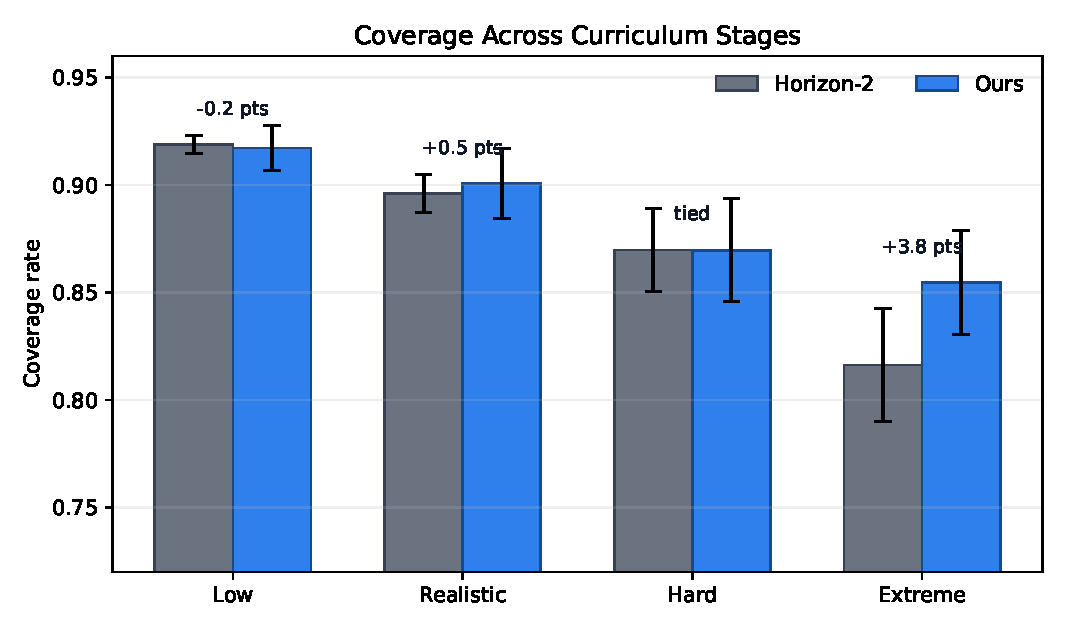
\includegraphics[width=\columnwidth]{figures/main_coverage_ours_vs_horizon2.pdf}
\caption{带分层95\%置信区间的阶段覆盖率。差异主要出现在Extreme阶段，且经多重比较校正后不再显著。}
\label{fig:coverage_zh}
\end{figure}

\begin{table}[t]
\caption{确定性与学习基线的覆盖率。方括号为分层95\%置信区间，$\pm$为评估种子标准差。}
\label{tab:baselines_zh}
\centering\tiny\setlength{\tabcolsep}{1.1pt}
\resizebox{\columnwidth}{!}{%
\begin{tabular}{@{}lcccc@{}}
\toprule
方法 & Low & Real. & Hard & Extreme\\
\midrule
本方法 & .917 [.906,.929] & .901 [.884,.922] & .870 [.844,.894] & .855 [.828,.881]\\
Horizon-2 & .919 [.906,.932] & .896 [.883,.910] & .870 [.847,.894] & .816 [.782,.849]\\
Horizon-3 & .917$\pm$.009 & .927$\pm$.025 & .860$\pm$.022 & .841$\pm$.060\\
风险感知 & .924 [.902,.953] & .901 [.885,.918] & .836 [.778,.876] & .863 [.833,.892]\\
最近优先 & .922$\pm$.011 & .887$\pm$.016 & .860$\pm$.026 & .789$\pm$.050\\
最老优先 & .914$\pm$.004 & .890$\pm$.014 & .883$\pm$.019 & .807$\pm$.032\\
距离--年龄 & .921$\pm$.016 & .896$\pm$.008 & .851$\pm$.020 & .801$\pm$.065\\
动态加权 & .927$\pm$.003 & .886$\pm$.023 & .865$\pm$.005 & .799$\pm$.045\\
ACO-TSP & .925$\pm$.006 & .893$\pm$.004 & .864$\pm$.033 & .754$\pm$.061\\
规划器集成 & .935$\pm$.012 & .899$\pm$.014 & .870$\pm$.003 & .814$\pm$.090\\
无残差 & .838 [.712,.915] & .776 [.667,.865] & .726 [.590,.837] & .687 [.585,.793]\\
Vanilla LSTM-PPO & .166 [.067,.286] & .130 [.048,.234] & .089 [.025,.181] & .061 [.017,.115]\\
\bottomrule
\end{tabular}}
\\[-2pt]
\raggedright\footnotesize 确定性方法采用相同环境种子和动作接口。Vanilla因训练协议存在混杂，仅作为带区间的描述性诊断，不作为因果基线。
\end{table}

\subsection{动作接口、服务代价与鲁棒性}
匹配的无残差策略保留观测、LSTM、H2预热、预测损失、服务奖励和训练预算，但输出绝对动作，且不含规划基准或保护器。该比较用于检验完整规划--残差动作接口。历史Vanilla同时改变残差组合、BC与预测，且未完成全预算独立调优，因此不作因果解释。

在Extreme阶段，相较H2，$0.038$的覆盖率增加伴随平均延迟增加$2.50$ s、p90增加$6.09$ s、平均活动热斑数增加$0.26$及严格SLA降低。在未见的更高密度条件下，本方法在Hard/Extreme获得.868/.850，H2获得.888/.825；区间重叠，因此仅作为鲁棒性证据。H3结果构成规划时域敏感性分析，不支持残差跨基础规划器迁移的结论。

\begin{table*}[t]
\caption{机制与服务证据：（a）匹配残差接口效应；（b）组件核算；（c）相对H2的覆盖率--服务诊断。}
\label{tab:diagnostic_panels_zh}
\centering\scriptsize
\begin{minipage}[t]{0.485\textwidth}
\centering
\textbf{（a）匹配残差接口效应}\\[2pt]
\setlength{\tabcolsep}{1.8pt}
\resizebox{\linewidth}{!}{%
\begin{tabular}{@{}lccccc@{}}
\toprule
阶段 & 完整方法 & 无残差 & $\Delta$ & $\Delta$区间 & $p_{\rm Holm}$\\
\midrule
Low & .917 & .838 [.712,.915] & +.079 & [.004,.202] & .029\\
Real. & .901 & .776 [.667,.865] & +.124 & [.036,.223] & .003\\
Hard & .870 & .726 [.590,.837] & +.144 & [.037,.268] & .011\\
Extreme & .855 & .687 [.585,.793] & +.168 & [.050,.285] & .003\\
\bottomrule
\end{tabular}}\\[3pt]
\textbf{（b）组件核算}\\[2pt]
\setlength{\tabcolsep}{1.6pt}
\resizebox{\linewidth}{!}{%
\begin{tabular}{@{}lccccccc@{}}
\toprule
变体 & 动作 & BC & 注意力 & 传递 & 预测 & 服务 & 保护\\
\midrule
完整方法 & H2+残差 & 是 & 是 & 是 & 是 & 是 & 是\\
无残差 & 绝对 & 是 & 是 & 是 & 是 & 是 & 否\\
无注意力 & H2+残差 & 是 & 否 & 是 & 是 & 是 & 是\\
无传递 & H2+残差 & 是 & 是 & 否 & 是 & 是 & 是\\
无预测 & H2+残差 & 是 & 是 & 是 & 否 & 是 & 是\\
无服务奖励 & H2+残差 & 是 & 是 & 是 & 是 & 否 & 是\\
Vanilla & 绝对 & 否 & 是 & 是 & 否 & 是 & 否\\
\bottomrule
\end{tabular}}
\end{minipage}\hfill
\begin{minipage}[t]{0.485\textwidth}
\centering
\textbf{（c）相对H2的覆盖率与服务诊断}\\[2pt]
\setlength{\tabcolsep}{2.0pt}
\resizebox{\linewidth}{!}{%
\begin{tabular}{@{}llrrrrrr@{}}
\toprule
阶段 & 方法 & 覆盖率 & 平均延迟(s) & p90(s) & 严格SLA & 积压 & $\Delta_u$\\
\midrule
Low & 本方法 & .917 & 12.54 & 24.15 & .181 & 2.30 & .0254\\
 & H2 & .919 & 12.16 & 23.72 & .191 & 2.28 & .0255\\
Real. & 本方法 & .901 & 16.04 & 29.70 & .147 & 2.84 & .0261\\
 & H2 & .896 & 16.52 & 29.45 & .131 & 2.82 & .0258\\
Hard & 本方法 & .870 & 19.59 & 38.10 & .127 & 3.49 & .0277\\
 & H2 & .870 & 19.23 & 35.44 & .121 & 3.43 & .0274\\
Extreme & 本方法 & .855 & 23.88 & 46.01 & .103 & 3.81 & .0289\\
 & H2 & .816 & 21.38 & 39.92 & .128 & 3.55 & .0277\\
\bottomrule
\end{tabular}}
\vspace{1pt}

\raggedright\footnotesize 平均和p90延迟以已覆盖热斑为条件；严格SLA以全部生成热斑为分母。积压为平均活动数，$\Delta_u$为每步平均动作变化。
\end{minipage}
\end{table*}

\begin{figure*}[t]
\centering
\begin{tabular}{cc}
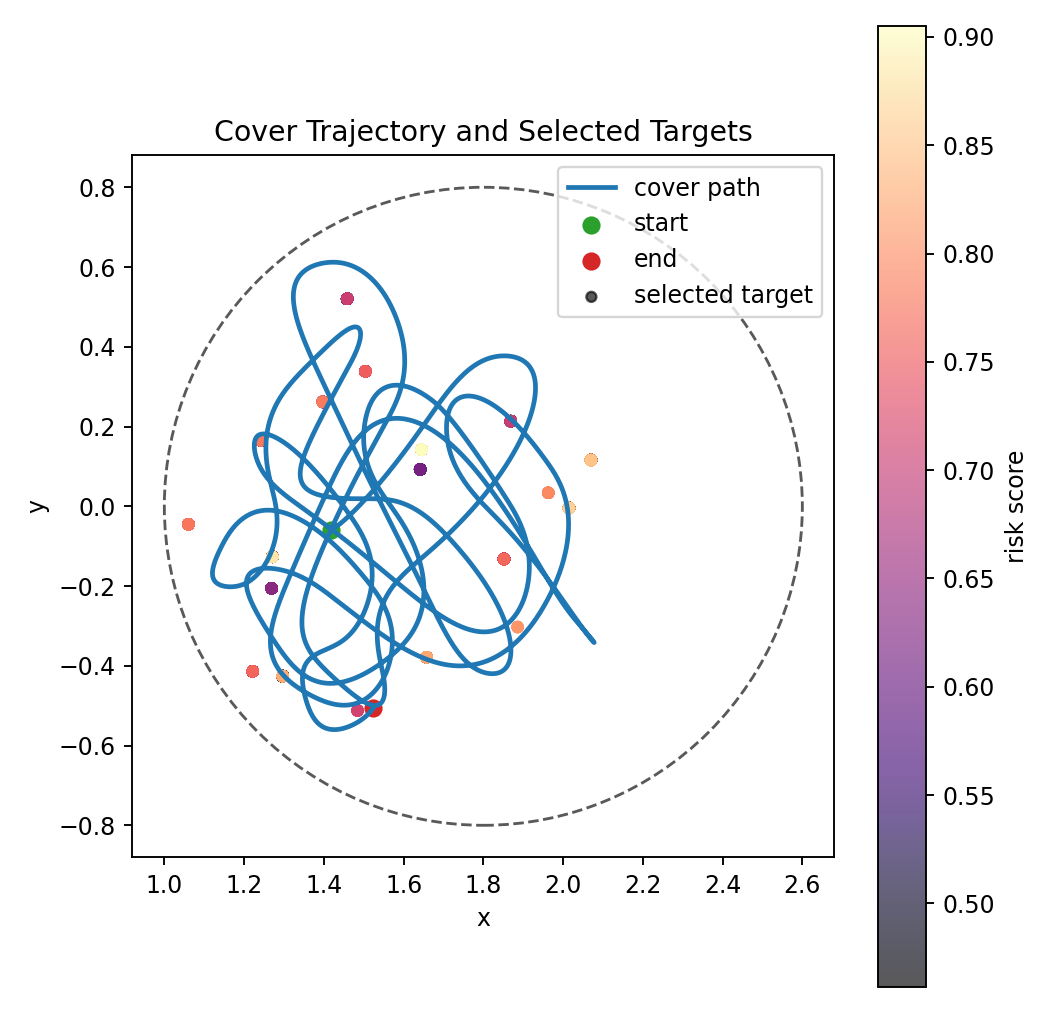
\includegraphics[width=0.25\textwidth]{figures/ours_realistic_trajectory.png} &
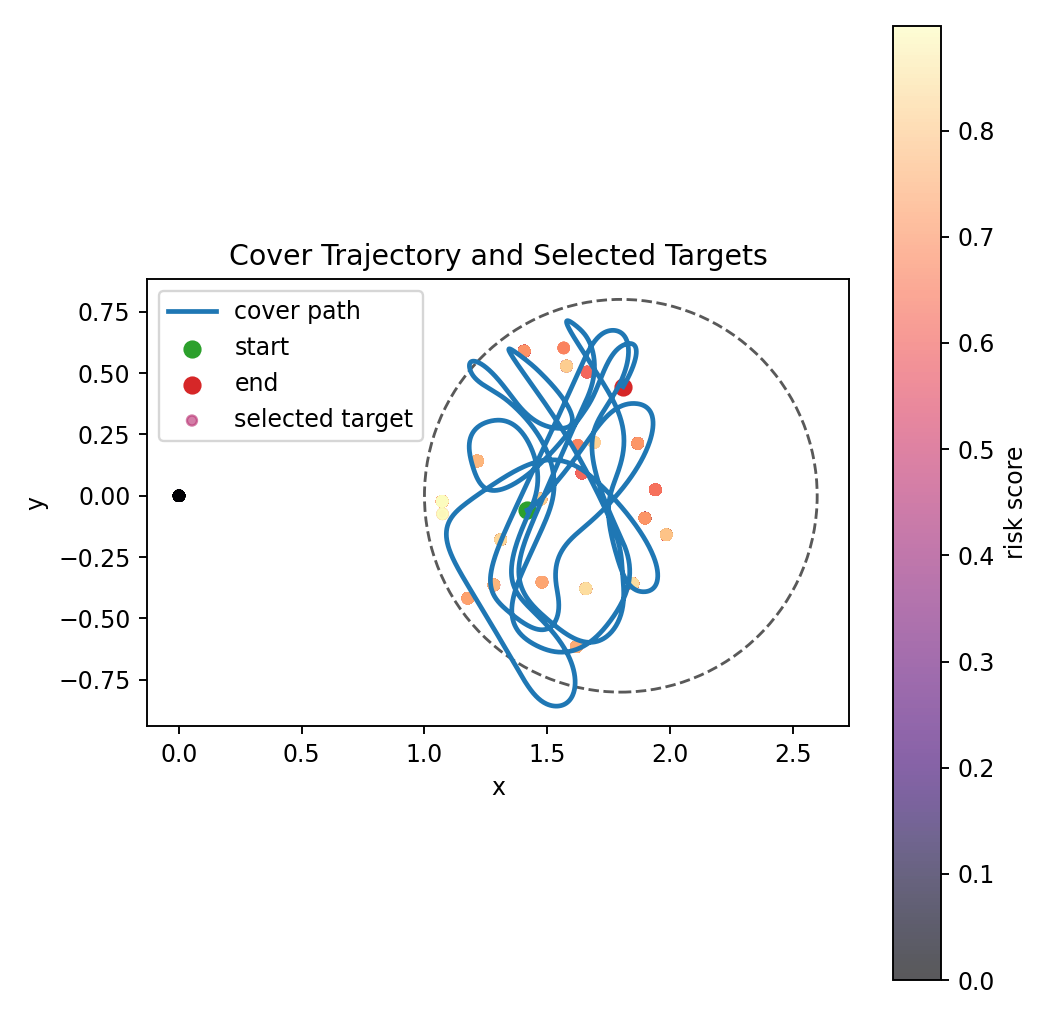
\includegraphics[width=0.25\textwidth]{figures/horizon2_realistic_trajectory.png}\\
（a）规划器引导残差PPO & （b）Horizon-2
\end{tabular}
\caption{留出Realistic场景的代表性轨迹。总体结论基于训练种子与评估种子的交叉单元。}
\label{fig:trajectory_zh}
\end{figure*}

\FloatBarrier
\section{讨论与结论}
匹配动作接口比较表明，完整规划--残差接口与覆盖率提升一致，但该结果不能证明本方法优于H2或风险感知启发式。前三阶段中H2与学习方法无统计可区分差异，Extreme差值在Holm校正前为正、校正后不显著。历史Vanilla同时改变残差组合、BC和预测，故仅作为描述性诊断；现有辅助消融也不能证明注意力、隐状态传递、预测或服务塑形分别产生独立增益。

H3检验的是确定性规划器容量，而非残差迁移，因为学习控制器以H2动作为条件。$0.05$ s间隔表示任务时间而非模型推理时间，固定窗口也不要求最终清空全部活动热斑。因此，本文证据适用于固定时域持续服务；终端排空评估、跨规划器残差迁移和硬件时序验证仍需后续完成。

\begingroup
\renewcommand{\footnotesize}{\tiny}
\makeatletter
\def\IEEEbibitemsep{-1pt}
\makeatother
\bibliographystyle{IEEEtran}
\bibliography{rl_robot_refs}
\endgroup

\end{document}
